\documentclass[12pt]{article}
\usepackage[shortlabels]{enumitem}
\usepackage{float}
\usepackage{xcolor}
\usepackage[a4paper, top=0.8cm, bottom=0.8cm, left=2cm, right=2cm]{geometry}
\usepackage{parskip}
\usepackage{setspace}
\usepackage{lmodern}
\usepackage[T1]{fontenc}
\usepackage[brazil]{babel}
\usepackage{hyperref}
\usepackage{graphicx}
\usepackage{amsmath}
\usepackage{amssymb}
\usepackage{amsfonts}
\usepackage{dsfont}
\usepackage{float}
\title{Prova 2 - Estatística - 2025.1}
\begin{document}
\date{}
\maketitle

1) (1,8 pontos) Uma  indústria de pequeno porte no setor de laticínios  está enfrentando sérios problemas em sua linha de produção.
 Estima-se que 30\% do leite recebido no estabelecimento apresente um resíduo indesejado específico que não está sendo detectado pelos testes físico-químicos realizados atualmente pelo laboratório dessa indústria. 

Como a empresa é pequena e possui recursos limitados, não possui acesso aos melhores testes do mercado para identificação desse novo resíduo contaminante,
mas consegue adquirir um teste que apresenta as seguintes características:
 
\begin{itemize}
    \item Se a amostra estiver contaminada, o teste apresenta resultado positivo, identificando a presença de contaminantes, com 70\% de chance.
    \item Se amostra não estiver contaminada, o teste apresenta resultado negativo, identificando ausência de contaminantes, com 80\% de chance.
\end{itemize}

O engenheiro responsável pelo laboratório dessa indústria realiza o teste em uma amostra do lote e o teste dá positivo. 
Sabendo disso, ele precisa tomar a decisão de rejeitar ou não o lote. 
Ele decide estabelecer que, caso a probabilidade dessa amostra realmente estar contaminada seja maior que 50\%, então o lote deve ser rejeitado.
Caso contrário, mesmo o teste dando positivo, ele aceita o lote. Dado esse cenário, o engenheiro deve rejeitar ou aceitar o lote de leite recebido? Justifique sua resposta com os cálculos necessários. 


\vspace{5px}

2) (2,65 pontos) Um dos jogos da loteria federal que vem se tornando popular ao longo dos últimos anos devido à sua aparente facilidade de ganho é a Lotofácil.
 Diferentemente da tradicional Mega-Sena, na Lotofácil existem apenas 25 números dos quais, na aposta comum, o jogador
deve marcar 15 números, pagando o valor de R\$ 3,00. O jogador recebe um prêmio relativo à quantidade de acertos, a seguir são listados os prêmios do último sorteio:
\begin{itemize}
    \item Prêmio ao acertar 15 números: 	$R\$ 1.764.882,05$
    \item Prêmio ao acertar 14 números: 	$R\$ 1.737,36$
    \item Prêmio ao acertar 13 números: 	$R\$ 30,00$
    \item Prêmio ao acertar 12 números: 	$R\$ 12,00$
    \item Prêmio ao acertar 11 números: 	$R\$ 6,00$ 
\end{itemize}

A seguir é apresentada uma imagem do cartão do jogo:

\begin{figure}[H]
    \centering
    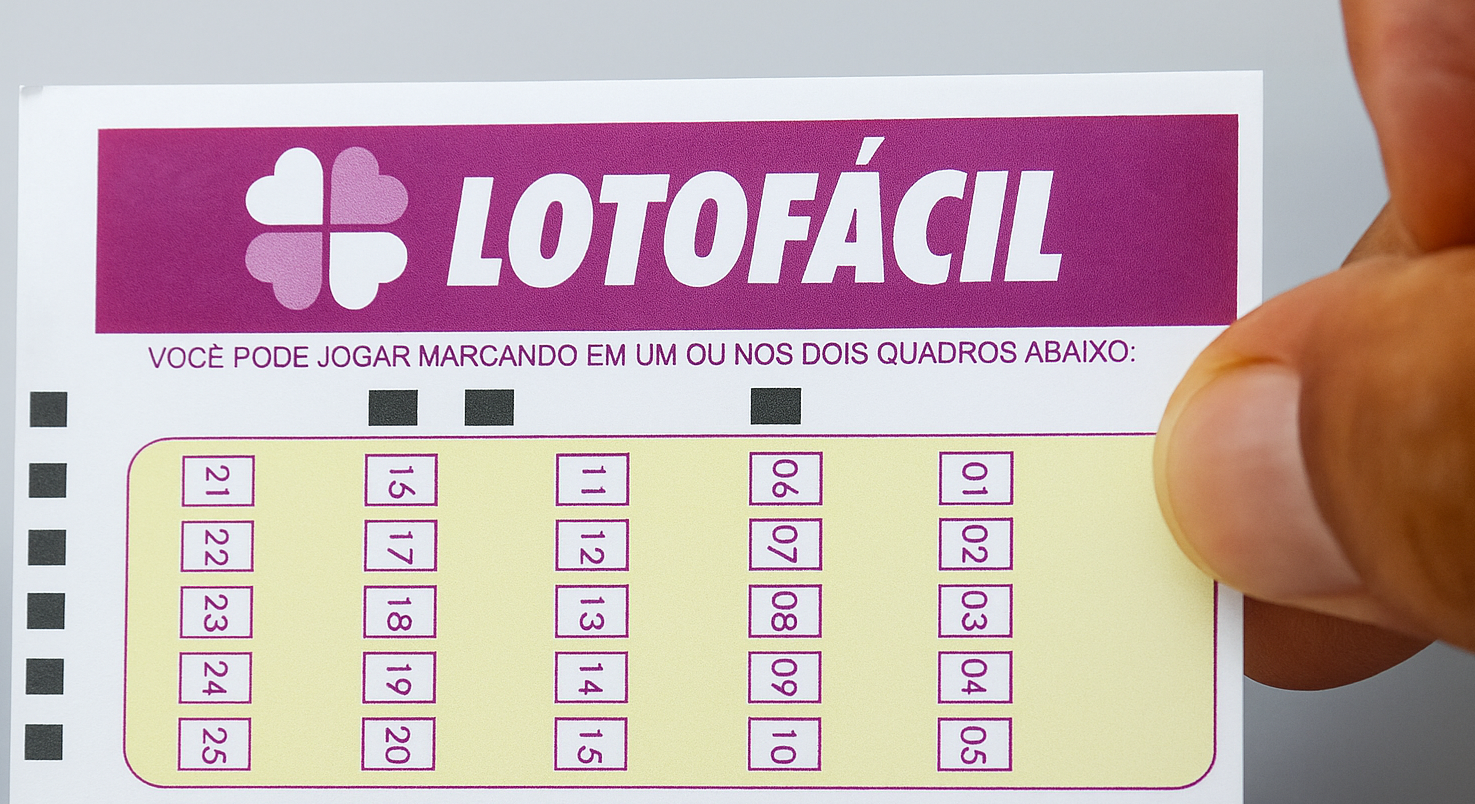
\includegraphics[width=0.5\linewidth]{figures/lotofacil.png}
\end{figure}

Sabendo disso responda:

\begin{enumerate}[a)]
    \item (1,9 pontos) Sabemos que, por ser um jogo da loteria federal, trata-se de um jogo em que não há fraude e, portanto, é um jogo justo nesse quesito. Entretanto, ao longo
    da disciplina, vimos que, atrelado ao surgimento da probabilidade, também surge o ato de verificar, por meio do uso de probabilidades, se um jogo aleatório 
    é justo. Dessa forma, considerando a aposta comum, é possível afirmar que, baseando-se nesse conceito de justiça, o jogo da Lotofácil é justo? Justifique sua resposta realizando os cálculos 
    necessários. 
    \item (0,75 pontos) Pierre, um jogador da Lotofácil, resolve adotar a seguinte estratégia para aumentar suas chances de ganho: Ele entra na internet e busca todos os números sorteados
    nos sorteios realizados ao longo do ano de 2024 e monta a seguinte tabela de frequência:
\begin{table}[H]
\centering
\caption{Frequência das dezenas da Lotofácil no ano de 2024}
\begin{tabular}{|c|c|c|}
\hline
\textbf{Dezena} & \textbf{Vezes} & \textbf{Frequência Relativa} \\ \hline
10 & 195 & 67.24\% \\ \hline
25 & 191 & 65.86\% \\ \hline
12 & 185 & 63.79\% \\ \hline
02 & 184 & 63.45\% \\ \hline
01 & 181 & 62.41\% \\ \hline
08 & 181 & 62.41\% \\ \hline
04 & 178 & 61.38\% \\ \hline
03 & 177 & 61.03\% \\ \hline
15 & 176 & 60.69\% \\ \hline
20 & 176 & 60.69\% \\ \hline
05 & 175 & 60.34\% \\ \hline
19 & 173 & 59.66\% \\ \hline
07 & 172 & 59.31\% \\ \hline
21 & 171 & 58.97\% \\ \hline
22 & 171 & 58.97\% \\ \hline
23 & 171 & 58.97\% \\ \hline
18 & 170 & 58.62\% \\ \hline
06 & 168 & 57.93\% \\ \hline
13 & 167 & 57.59\% \\ \hline
14 & 166 & 57.24\% \\ \hline
09 & 165 & 56.90\% \\ \hline
24 & 165 & 56.90\% \\ \hline
11 & 164 & 56.55\% \\ \hline
16 & 164 & 56.55\% \\ \hline
17 & 164 & 56.55\% \\ \hline
\hline
\end{tabular}
\end{table}

Pierre acredita que a probabilidade de um número ser sorteado está relacionada à frequência com que ele apareceu em sorteios anteriores, ou seja, considera que a probabilidade é equivalente à frequência relativa observada. 
Assim, os números mais frequentes seriam, segundo ele, os mais prováveis de serem sorteados. Dessa forma, com o objetivo de aumentar suas chances de ganhar, ele simplesmente escolhe marcar, no cartão de aposta, os 15 primeiros números da tabela apresentada acima.

Dado esse cenário, responda:

\begin{enumerate}[i)]
    \item (0,25 pontos) Qual interpretação da probabilidade Pierre está usando? 
    \item (0,5 ponto) A interpretação adotada por Pierre é a mais adequada para o contexto do problema? Se a resposta for não, qual seria a interpretação mais adequada e por que? Se for sim, diga o motivo. 
\end{enumerate}

\vspace{5px}



% 3) Carlos trabalha em um restaurante. Após vencerem juntos um bolão da Mega-Sena e dividirem igualmente o prêmio de R\$ 40 milhões, os 6 colegas de Carlos pedem demissão da empresa. Carlos, que não havia participado do bolão, permanece no setor e é promovido a gerente.

% A empresa autoriza a contratação de \textbf{6 novos funcionários}, mas o processo levará cerca de 6 meses. Antes mesmo das contratações, Carlos, preocupado com o orçamento apertado e com possíveis \textit{gastos com bolos, refrigerantes e decoração}, decide que não irá comemorar os aniversários individualmente.

% Para evitar custos semanais com festas repetidas, ele estabelece o seguinte critério:

% \begin{quote}
% \textit{“Se a chance de pelo menos dois dos 7 funcionários (ele mais os 6 futuros) fazerem aniversário na mesma semana for maior ou igual a 20\%, então só haverá uma comemoração por mês. Caso contrário, posso considerar comemorações semanais.”}
% \end{quote}

% \begin{enumerate}[a)]
%     \item Sabendo que há 52 semanas no ano e assumindo que os aniversários são distribuídos aleatoriamente ao longo das semanas, \textbf{qual decisão Carlos deve tomar?}
%     \item Carlos sabe que a empresa não funciona na semana que sucede o Natal. Logo, se ele decidir comemorar os aniversários semanalmente e alguém fizer aniversário nessa semana, não há comemoração. Qual a probabilidade de que pelo menos dois dos 7 funcionários façam aniversário na semana que sucede o Natal. Obs: Assuma que a data de aniversário de Carlos pode ocorrer em qualquer semana do ano, inclusive na semana que sucede o Natal.
% \end{enumerate}


3) (2,5 pontos) Uma distribuição contínua bastante importante e adotada na geração de números aleatórios em programas computacionais é a Distribuição Uniforme Contínua. 
Dizemos que se uma variável aleatória $X$ segue a distribuição uniforme contínua em um intervalo $[a,b]$ (Notação: $X \sim U([a,b])$) com $b > a$, se ela assume valores
no conjunto $[a,b]$ e sua função densidade de probabilidade é dada por:

$$f(x) = \begin{cases}
\dfrac{1}{b-a}, & \text{ se } a \leq  x \leq b \\
0, & \text{ caso contrário}
\end{cases}$$

Sabendo disso responda:

\begin{enumerate}[a)]
    \item(1 ponto) Mostre que se $X \sim U([a,b])$ então $\mathbb{E}[X] = \dfrac{a+b}{2}$ e $Var(X) = \dfrac{(b-a)^2}{12}$
    \item(1,5 pontos) Além da Distribuição Uniforme Contínua, também existe a Distribuição Uniforme Discreta. 
    Dizemos que uma variável aleatória $Y$ segue a distribuição uniforme discreta em um conjunto $\{a, a+1, a+2, \dots, b\}$ (Notação: $Y \sim \mathcal{U}\{a,b\}$) com $b > a$ se $Y$ assume valores no conjunto enumerável
    $\{a, a+1, a+2, \dots, b\}$ e sua função de probabilidade é dada por:

    $$p_{Y}(y) = \dfrac{1}{b-a+1}  \text{ se } y \in \{a, a+1, \dots, b\}$$

    Sabendo disso e dados os conceitos discutidos em sala acerca de variáveis aleatórias, responda:
    \begin{enumerate}[i)]
        \item(0,3 pontos) O que é uma variável aleatória. 
        \item(0,2 pontos)Explique a diferença entre uma variável aleatória discreta e uma contínua.
        \item (0,3 pontos) Explique o que é uma função de probabilidade (Explique seu aspecto funcional, incluindo os requisitos para uma função ser função de probabilidade).
        \item (0,2 pontos)Suponha que $T \sim U([1,6])$ e  $V \sim \mathcal{U}\{1,6\}$, obtenha $\mathds{P}(T=2)$ e $\mathds{P}(V=2)$.
        \item (0,3 pontos) Suponha que $T \sim U([1,6])$ e  $V \sim \mathcal{U}\{1,6\}$, obtenha $F_T(4)$ e $F_{V}(4)$.
        \item (0,2 pontos) Dê um exemplo de evento do mundo real que poderia ser modelado por uma variável aleatória que siga a distribuição uniforme discreta e outro que poderia ser modelado por uma que siga a uniforme contínua.Obs: O exemplo não pode ser o mesmo do enunciado da questão.
    \end{enumerate}
\end{enumerate}

\vspace{5px}
4) (2,2 pontos) Você é o Engenheiro responsável por um laboratório de controle de qualidade que está avaliando amostras de leite cru fornecido por diferentes
 produtores da região. Uma das análises realizadas é o teste de crioscopia, que mede o ponto de congelamento do leite. 

Para verificar se os fornecedores estão adicionando água ao leite, você selecionou uma amostra aleatória de 36 lotes de leite e obteve uma média do ponto de 
congelamento igual a \( -0{,}533\,^\circ\mathrm{C} \).

Estudos anteriores do laboratório indicam que a variabilidade do ponto de congelamento do leite é bem conhecida, com desvio padrão populacional  $\sigma = 0{,}072\,^\circ\mathrm{C}$.
Admita que a variável aleatória associada ao ponto de congelamento seja aproximadamente normal.

\begin{enumerate}
    \item(0,5 pontos) Construa um intervalo de confiança com 95\% de confiança para a média real do ponto de congelamento do leite entregue pelos fornecedores.

    \item(0,6 pontos) Você decide mostrar o intervalo de confiança obtido para Leôncio, o técnico do laboratório. Ao ler seu resultado, Leôncio profere a seguinte frase para você:
    
    \begin{quote}
\textit{“Baseado no intervalo que você me mostrou, podemos dizer que existe uma probabilidade de 95\% de que a média verdadeira do ponto de congelamento do leite recebido esteja compreendida dentro desse intervalo ”}
\end{quote}

    Você concorda com a afirmação do técnico do laboratório? Justifique. 

    \item (0,6 pontos) O que ocorreria com o intervalo calculado na questão $a$ se o tamanho da amostra aumentasse? E se o nível de confiança aumentasse?
    

    \item (0,5 ponto) Se o laboratório desejasse uma margem de erro de no máximo \( 0{,}005\,^\circ\mathrm{C} \) para a média, mantendo o mesmo nível de confiança e desvio padrão, qual deveria ser o tamanho mínimo da amostra?
\end{enumerate}

\vspace{5px}

5)(1,1 pontos) Sejam $A$ e $B$ dois eventos em um mesmo espaço amostral. Responda:

\begin{enumerate}[a)]
    \item (0,3) O que significa dizer que $A$ e $B$ são mutuamente excludentes(ou exclusívos)?
    \item (0,3) O que significa dizer que $A$ e $B$ são independentes? Dizer que $A$ é independente de $B$ implica dizer que $B$ é independente de $A$?
    \item (0,5) Se $A$ e $B$ são mutuamente excludentes(ou exclusívos), logo também são independentes? O contrário é valido?
\end{enumerate}
Informações úteis: 
\begin{itemize}
    \item $\dfrac{25!}{15!10!} = 3268760$
    \item $\binom{15}{12} = 455$
    \item $\binom{15}{11} = 1365$
    \item  $\binom{10}{4} = 210$
    \item $\dfrac{1}{\binom{25}{15}} \approx 3,06 \cdot 10^{-7}$
    \item $\dfrac{150}{\binom{25}{15}} \approx 4,59 \cdot 10^{-5}$
    \item $\dfrac{4725}{\binom{25}{15}} \approx 1,44 \cdot 10^{-3}$
    \item $\dfrac{54600}{\binom{25}{15}} \approx 5,01 \cdot 10^{-2}$
    \item $\dfrac{286650}{\binom{25}{15}} \approx 8,77 \cdot 10^{-2}$
\end{itemize}
% 5)(1,5 pontos) Diga se as afirmações a seguir são verdadeiras ou falsas e justifique matematicamente suas respostas. 

% \begin{enumerate}[a)]
%     \item (0,2 pontos) Dados dois eventos $A$ e $B$. Se $A$ e $B$ são mutuamente excludentes então também são independentes. 
%     \item (0,3 pontos) Dados dois eventos $F$ e $G$ tal que $F \subset G$, portanto, $\mathds{P}(G|F) = 1$
%     \item (1 ponto) Dados dois eventos $A$ e $B$, se $\mathds{P}(A|B) =1$ então $\mathds{P}(B^c|A^c) =1$
% \end{enumerate}


\end{document}